\documentclass[aspectratio=43,12pt]{beamer}

\usepackage{moresize}
\usepackage{siunitx}
\usepackage{xspace}

\usepackage{tikz}
\usetikzlibrary{positioning}
\usetikzlibrary{shapes,arrows,backgrounds,fit,shapes.geometric,calc,petri}
\usetikzlibrary{pgfplots.groupplots}
\usetikzlibrary{arrows.meta}
\usepackage{pgfplots}
\usepackage{pgfplotstable}

\usepackage{listings}
\usepackage{lstautogobble}
\usepackage{color}

\lstset{
    language=[ANSI]C++,
    basicstyle=\scriptsize,
    identifierstyle=\color{blue}\scriptsize,
    keywordstyle=\color{purple}\scriptsize,
%    commentstyle=\color{green!30!black}\bf\small\ttfamily,
    showspaces=false,
    showstringspaces=false,
    breaklines=true
}

\newcommand{\lst}[1]{\lstinline!#1!}

% Increase spacing in lists and enumerations.
% Source: http://tex.stackexchange.com/questions/225736/latex-beamer-define-itemsep-globally
\usepackage{xpatch}
\xpatchcmd{\itemize}
  {\def\makelabel}
  {\ifnum\@itemdepth=1\relax
     \setlength\itemsep{1ex}% separation for first level
   \else
     \ifnum\@itemdepth=2\relax
       \setlength\itemsep{0.5ex}% separation for second level
     \else
       \ifnum\@itemdepth=3\relax
         \setlength\itemsep{0.5ex}% separation for third level
   \fi\fi\fi\def\makelabel
  }
 {}
 {}

% Theme works only with a 4:3 aspect ratio
\usetheme{CSCS}

% define footer text
\newcommand{\footlinetext}{\xmc{}}

% Select the image for the title page
\newcommand{\picturetitle}{cscs_images/image3.pdf}

\newcommand{\xmc}{\texttt{xmc}\xspace}

\newcommand{\ttilde}{\char`\~}

\newcommand{\subheading}[1]{{\large #1}}
\newcommand{\TODO}[1]{\textcolor{red}{TODO: \bf #1}}

% Please use the predifined colors:
% cscsred, cscsgrey, cscsgreen, cscsblue, cscsbrown, cscspurple, cscsyellow, cscsblack, cscswhite

% colour rebel!
\definecolor{light-grey}{gray}{0.6}

\author{Sam Yates, CSCS}
\title{\xmc}
\subtitle{\xmc: modelling spiking multi-compartment networks at exascale}
\date{14 June 2017}
\begin{document}

% TITLE SLIDE
\cscstitle

% Talk notes:
% 1. Presenting work on xmc.
% 2. xmc is a joint project between CSCS, BSC, J"ulich
% 3. xmc is a platform for m.c. network simulators to run on HPC systems.

%--
\begin{frame}
\frametitle{What is \xmc?}
\vfill
\xmc{} is a project to develop a library:

\vfill
\begin{itemize}
\item for simulating multi-compartmental neurons;
\item designed for current and future HPC systems;
\item which is highly customizable.
\end{itemize}
\vfill

\centering 
\vspace{4ex}
% dodgy by-hand scaling

\includegraphics[height=2.8em]{logos/cscs_logo.pdf}
\hspace{15mm}

\includegraphics[height=3em]{logos/julich_logo.pdf}
\hspace*{5mm}
\\[1.4em]

\includegraphics[height=2.9em]{logos/bsc_logo.pdf}\\
\end{frame}


% Talk notes:
% Motivation:
% 1. No more free lunch: single threaded performance plateau.
% 2. Processors moving to 'throughput' oriented highly parallel accelerators
%    (GPUs) and many-core architectures e.g. Xeon Phi.
% 3. These demand differening and specialized implementations.
% (slides below direct from Bernstein 2016 presentation)

%--
\begin{frame}
\frametitle{The limits of frequency}

\vfill
Microprocessor transistor counts have grown
exponentially over a very long time frame.

\vfill
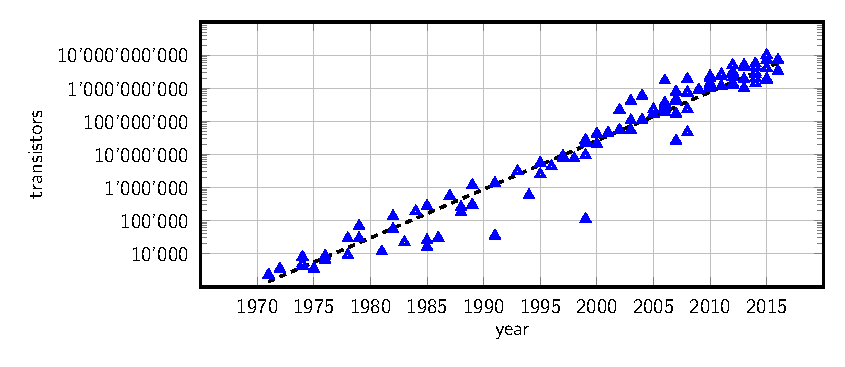
\includegraphics[height=0.5\textheight]{transistors.pdf}
\vfill
\end{frame}

%--
\begin{frame}
\frametitle{The limits of frequency}

\vfill
Processor clock speed growth suddenly slowed around 2004.

\vfill
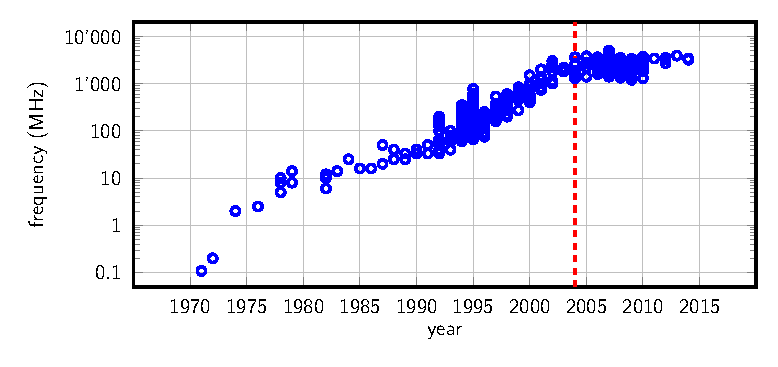
\includegraphics[height=0.45\textwidth]{frequency.pdf}

\vfill
\centering
\textbf{Problem:} $\quad\hbox{power}\ \propto\ \hbox{frequency}^3$

\vfill
\end{frame}


\begin{frame}
\frametitle{The limits of frequency}
\vfill
Single-thread performance growth also slows.

\vfill
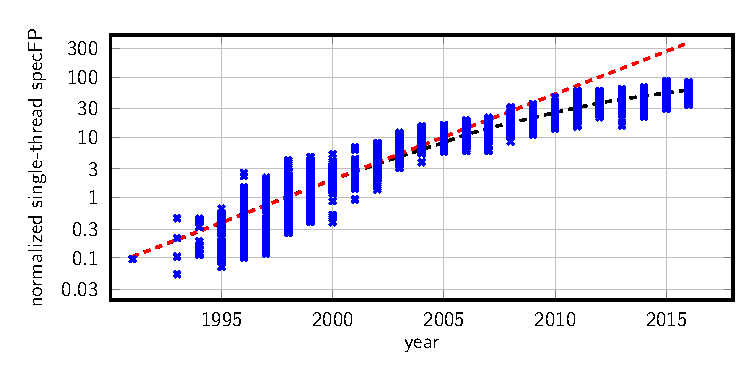
\includegraphics[height=0.5\textwidth]{fp-performance.pdf}

\vfill
\hfill{\scriptsize Analysis thanks to Jeff Preshing, http://preshing.com}
\end{frame}

%--
\begin{frame}
\frametitle{New HPC architectures}

\vfill
New performance gains primarily from:

\vfill
\begin{itemize}
\item Highly parallel architectures (e.g. Intel KNL).
\item Wider vector operations (e.g. AVX512).
\item Specialized accelerator hardware: GPU, FPGA.
\end{itemize}

\vfill
Challenge: optimizing multiple simulators for multiple architectures.
% Talk point: opportunity for a library to reduce this complexity, making
% the problem additive instead of multiplicative.
\vfill
\end{frame}

%--


\begin{frame}
\frametitle{\xmc{} design requirements}


The \xmc{} library must allow:
\begin{enumerate}
\item
Performance portability
\pause
\begin{itemize}
\item Target-independent abstractions but:
\item Target-specific data structures and code.
\end{itemize}
\item
\pause
Scalability
\pause
\begin{itemize}
% Talk point; model size prop. nodes; memory per node roughly constant.
\item Distributed model construction.
\item Constrained communication costs.
\end{itemize}
\pause
\item
Extensibility
\pause
\begin{itemize}
\item New cell models.
\item New hardware architectures.
\item New numerical solvers \dots
\end{itemize}
\end{enumerate}

\end{frame}

% Talk notes:
% 1. Introduce architecture as mechanisms for achieving these aims.
% 2. Start with user-side extensibility: cell types, recipe, NMODL.
% 2b. Show connection with scalability, perf port.

% Talk point: software archictecture central to achieve these aims.
% 1. Front-end abstractions: recipes and cell types.

\begin{frame}
\frametitle{Model abstraction}

Models are described by a \textit{recipe}.\\
\vfill
Recipes take a cell number and give:
\begin{enumerate}
\item The \textit{type} of cell it is.
\item The number of spike \textit{targets} it has.
\item The number of spike \textit{sources} it has.
\item The list of connections to its targets from other cells.
\item A cell-type specific description of the cell.
\end{enumerate}

Descriptions and connection lists may be expensive, so are only
computed when requested.
\vfill
We are working with simulator developers and users to ensure
the compatibility of this model.
\end{frame}

\begin{frame}
\frametitle{Cell types}
Cable neuron:
\begin{itemize}
\item Piece-wise linear morphology.
\item Density channels and point synapses described in NMODL.
\item Any number of spike sources (typically one).
\end{itemize}

\vfill
Fixed-frequency artificial spike sources:
\begin{itemize}
\item Spiking frequency.
\item Activity start and stop times.
\item One spike source, no spike targets.
\end{itemize}

\vfill
More in development \dots
\end{frame}

\begin{frame}
\frametitle{Cell groups}

\vfill
Cell groups represent the implementation of multiple cells of the same type.
\vfill
\begin{center}
\begin{tikzpicture}[xscale=2.5, yscale=0.8]
    \path
        node at (0,2)  { \bf cell-type }
        node at (0,1)  { $\times$ }
        node at (0,0)  { \bf numerical scheme }
        node at (0,-1) { $\times$ }
        node at (0,-2) { \bf device implementation };
    %\draw (1,-2.5) -- (1,2.5);
    \path
        node at (2,3) [rectangle, draw, opacity=0] { fvm-gpu group }
        node at (2,2) [red, opacity=0] { cable neuron }
        node at (2,1) [red, opacity=0]  { $\times$ }
    node at (2,0) [red, opacity=0]  { finite volume }
        node at (2,-1) [red, opacity=0] { $\times$ }
        node at (2,-2) [red, opacity=0] { GPU/CUDA };
    \path node at (0,-3) {};
\end{tikzpicture}
\end{center}
\vfill

\end{frame}

\begin{frame}
\frametitle{Cell groups}

\vfill
Cell groups represent the implementation of multiple cells of the same type.
\vfill
\begin{center}
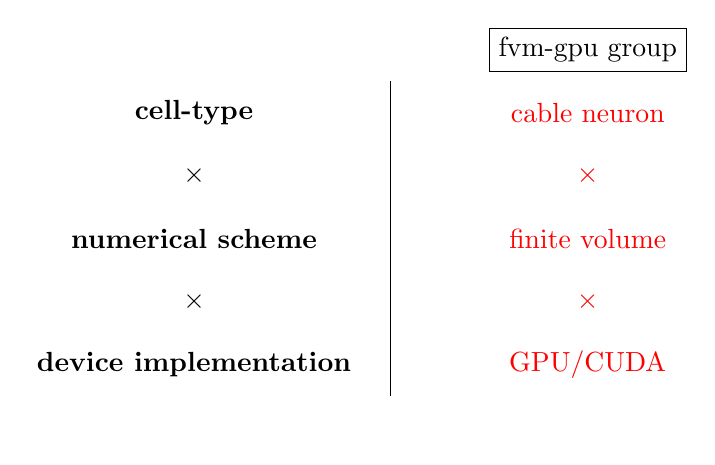
\begin{tikzpicture}[xscale=2.5, yscale=0.8]
    \path
        node at (0,2)  { \bf cell-type }
        node at (0,1)  { $\times$ }
        node at (0,0)  { \bf numerical scheme }
        node at (0,-1) { $\times$ }
        node at (0,-2) { \bf device implementation };
    \draw (1,-2.5) -- (1,2.5);
    \path
        node at (2,3) [rectangle, draw] { fvm-gpu group }
        node at (2,2) [red] { cable neuron }
        node at (2,1) [red]  { $\times$ }
    node at (2,0) [red]  { finite volume }
        node at (2,-1) [red] { $\times$ }
        node at (2,-2) [red] { GPU/CUDA };
    \path node at (0,-3) {};
\end{tikzpicture}
\end{center}
\vfill
\end{frame}

\begin{frame}
\frametitle{Why recipes and cell groups?}

Extensible:
\begin{enumerate}
\item Allows arbitrary new sorts of `cell'.
\item Multiple, independent numerical implementations per class.
\item Concrete cells per group is a runtime parameter.
\end{enumerate}

% Talk point: add different discretization schemes;
% Tune group size for hardware, i.e. very wide for gpu.

All cell groups share the same communication and control infrastructure.

\vfill
Scalable model building:
\begin{enumerate}
\item Recipes allow \textit{functional} model descriptions.
\item Work per node proportional to cells per node.
\end{enumerate}
\vfill
\end{frame}

\begin{frame}
\frametitle{Weak scaling of network construction}
\begin{itemize}
\item
300 compartments, 2000 synapses per cell.
\item
10,800 cells over 36 threads per rank.
\item
1 rank per 18-core Broadwell socket.
\end{itemize}

\includegraphics[width=\textwidth]{network-weak.pdf}
\vfill

\centering
Max 14\% increase to 1024 nodes, then flat.
\vfill
\end{frame}

\begin{frame}
\frametitle{Cells per group}

How many cells per group?

\pause
\hspace{4cm} \textit{Depends on optimal working set size.}
\vfill
\begin{itemize}
\item CPU: cell group data should fit in cache.
\item GPU: cell group data should aim to maximize data parallelism.
\end{itemize}
\end{frame}

%****************  BENCHMARKING  ****************
% set some reasonable default options for plots in this section
\pgfplotsset{every axis/.append style={
    legend style={font=\scriptsize},
    label style={font=\footnotesize},
    tick label style={font=\scriptsize},
    ylabel near ticks,
    xlabel near ticks
}}

\begin{frame}
\frametitle{Optimizing for cache size}

\centering
\vfill
Simulating 4068 cells for 50\,ms on one 18-core Broadwell CPU.
\vfill
\begin{tikzpicture}
    \begin{axis}[
    height=0.4\textwidth,
    width=\textwidth,
    ymin=0,ymax=10,
    xmin=1,xmax=64,
    xtick={1, 8, 16, 24, 32, 40, 48, 56, 64},
    xticklabels={1, 8, 16, 24, 32, 40, 48, 56, 64},
    ytick={2, 4, 6, 8},
    yticklabels={$2.0$, $4.0$, $6.0$, $8.0$},
    ylabel=Time (s),
    xlabel=Cells per cell group,
    legend style = {at={(0,1)}, anchor=north west},
    grid=major]
    \addplot[color=blue, mark=o,mark size=2,very thick] table[x=groupsize,y=walltime]
        {./x86_cache.tbl};
    \end{axis}
\end{tikzpicture}

\vfill
Fewer cells per group is faster: data for more than 16 cells no longer fits in cache.
\vfill
\end{frame}

\begin{frame}
\frametitle{Time to solution scaling with model size}

\centering
\vfill
Wall-clock time for 20\,ms simulation on CPU (one cell per group) and GPU (one group for all cells).
\vfill

\begin{tikzpicture}
    \begin{loglogaxis}[
    height=0.4\textwidth,
    width=\textwidth,
    xmin=1024,xmax=65536,
    %ymin=0.01,ymax=100,
    xtick={1, 8, 16, 24, 32, 40, 48, 56, 64, 128, 256, 512, 1024, 2048, 4096, 8192, 16384, 32768, 65536},
    xticklabels={1, 8, 16, 24, 32, 40, 48, 56, 64, 128, 256, 512, 1024, 2048, 4096, 8192, 16384, 32768, 65536},
    ylabel=Time (s),
    xlabel=Cells,
    legend style = {at={(0,1)}, anchor=north west},
    grid=major]
    \addplot[color=blue, mark=o,mark size=1, very thick] table[x=cells,y=cpu300]
        {./x86_vs_gpu_single_node.tbl};
    \addplot[color=red, mark=o,mark size=1, very thick] table[x=cells,y=gpu300]
        {./x86_vs_gpu_single_node.tbl};
    \legend{2$\times$18 core Broadwell, 1$\times$P100 GPU};
    \end{loglogaxis}
\end{tikzpicture}
\vfill
Linear scaling with CPU, but GPU requires large working set before achieving good throughput.
\vfill
\end{frame}

% Omitting this slide from talk: awkward to discuss matrix solver vs. parallel mechanism performance,
% especially given that matrix solve is WIP.
%
%\begin{frame}
%    \frametitle{GPU speedup as function of model size}
%
%    \begin{center}
%        {\small GPU speedup relative to multicore for a 20\,ms as the model size increases on a single node. 2000 synapses per cell.}
%    \end{center}
%        \vfill
%
%    \begin{tikzpicture}
%        \begin{semilogxaxis}[
%            height=0.4\textwidth,
%            width=\textwidth,
%            xmin=1024,xmax=65536,
%            %ymin=0.01,ymax=100,
%            xtick={1, 8, 16, 24, 32, 40, 48, 56, 64, 128, 256, 512, 1024, 2048, 4096, 8192, 16384, 32768, 65536},
%            xticklabels={1, 8, 16, 24, 32, 40, 48, 56, 64, 128, 256, 512, 1024, 2048, 4096, 8192, 16384, 32768, 65536},
%            ylabel=gpu speedup,
%            xlabel=cells,
%            legend style = {at={(1,0)}, anchor=south east},
%            grid=major]
%        \addplot[color=blue, mark=o,mark size=1, very thick]
%            table[x=cells,y expr=\thisrow{cpu300}/\thisrow{gpu300}]
%            {./x86_vs_gpu_single_node.tbl};
%        \addplot[color=red, mark=o,mark size=1, very thick]
%            table[x=cells,y expr=\thisrow{cpu30}/\thisrow{gpu30}]
%            {./x86_vs_gpu_single_node.tbl};
%        \addplot[color=black, very thick]
%            coordinates {(1, 1) (100000, 1)};
%        \legend{300 compartments/cell, 30 compartments/cell, break even};
%
%        \end{semilogxaxis}
%    \end{tikzpicture}
%
%    Time to solution on a single node (2$\times$BW18 vs P100 GPU) as the number size of the model is increased from 1k to 65k. Models with less complex cells scale better on GPU for lower cell counts\footnote{Note that the GPU version is not as well optimsed as the CPU.}.
%\end{frame}
%

\begin{frame}
\frametitle{Code generation}

Two problems:
\begin{enumerate}
\item Efficient cell state integration performance depends on
hardware-specific implementations.
\item Extensibility demands that new ion channels or synapse
models can be provided by simulator users.
\end{enumerate}
\vfill
It is not practical to explicitly implement optimized code for
each possible mechanism on each extant platform.
\vfill
\pause
Solution: use a DSL to describe mathematics, and generate
optimized code from that for each platform.
% Talk point: again avoids multiplicative growth in implementation effort.

\vfill
\pause
\xmc{} implements a subset of NEURON'S mechanism description languange \emph{NMODL}.
%(Hines, M. L. and Carnevale, N. T. (2000). Expanding NEURON's repertoire of mechanisms with NMODL. \emph{Neural Computation}, 12(5), 995--1007).
\end{frame}

\begin{frame}[fragile]
\frametitle{NMODL example}

\centering
Double-exponential synapse state
\vfill

\begin{columns}[T]
\begin{column}{0.5\textwidth}
\centering
    {\small NMODL}
\begin{lstlisting}[frame=single,language={}]
DERIVATIVE state {
    A' = -A/tau1
    B' = -B/tau2
}
\end{lstlisting}
\end{column}

\begin{column}{0.5\textwidth}
\centering
    {\small Non-vectorized generated code}
\begin{lstlisting}[frame=single]
for (int i_ = 0; i_ < n_; ++i_) {
    value_type dt = vec_dt[i_];
    value_type ll2_, ll1_, a_0_, ll0_, ll3_, a_1_;
    a_0_ = -1/tau1[i_];
    ll2_ = a_0_*dt;
    ll0_ = (1+0.5*ll2_)/(1-0.5*ll2_);
    A[i_] = A[i_]*ll0_;
    a_1_ = -1/tau2[i_];
    ll3_ = a_1_*dt;
    ll1_ = (1+0.5*ll3_)/(1-0.5*ll3_);
    B[i_] = B[i_]*ll1_;
}
\end{lstlisting}
\end{column}
\end{columns}
\end{frame}

\begin{frame}
\frametitle{Spike exchange}

\vfill
Cells are coupled via spike exchange --- spike propagation delay allows
cell state to be integrated independently up to some $\Delta T$.
\vfill

\xmc{} `communicator':
\begin{itemize}
\item Wraps underlying communication library (e.g. MPI).
\item Pre-process and broadcast locally generated spikes.
\item Deliver global list of spikes to local cell groups.
\end{itemize}
\vfill

Two key concerns for distributed exchange:
\begin{enumerate}
\pause
\item How to avoid communication latency?
\pause
\item How to scalably route spike information?
\end{enumerate}
\vfill
\end{frame}

\begin{frame}
\frametitle{Overlapping communication}

\centering
$\Delta T$ = minimum spike propagation delay.
\vfill
    \hspace{-50pt}
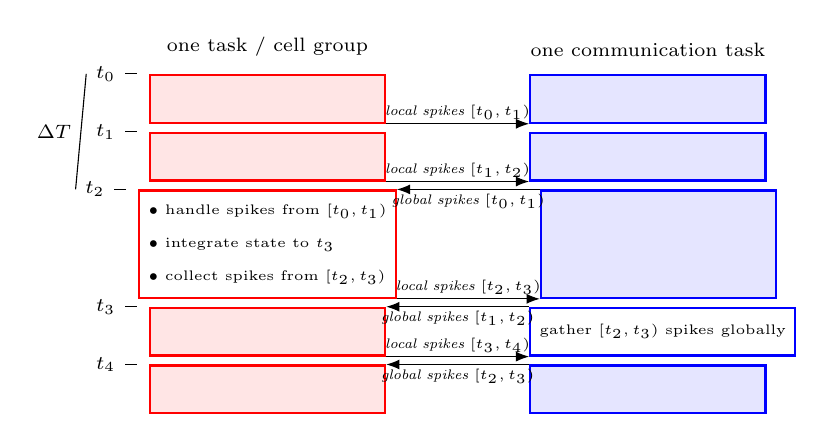
\begin{tikzpicture}
    [procae/.style={rectangle, draw=red, fill=red!10, thick, minimum height=4ex, minimum width=8.5em},
     procat/.style={rectangle, draw=red, thick, minimum height=4ex, minimum width=8.5em},
     procbe/.style={rectangle, draw=blue, fill=blue!10, thick, minimum height=4ex, minimum width=8.5em},
     procbt/.style={rectangle, draw=blue, thick, minimum height=4ex, minimum width=8.5em},
     tn/.style={minimum width=1em, align=left}]

    \node [procae] (y)  {};
    \node [procbe, right=12ex of y] (z) {};
    \path [-Latex] (y.south east) edge node [above=-2pt] {\tiny\it local spikes $[t_0, t_1)$} (z.south west);
    \node [procae, below=1mm of y] (a)  {};
    \node [procbe, right=12ex of a] (b) {};
    \path [-Latex] (a.south east) edge node [above=-2pt] {\tiny\it local spikes $[t_1, t_2)$} (b.south west);
    \node [procat, below=1mm of a, minimum height=9ex, align=left] (c) {
    \tiny $\bullet$ handle spikes from $[t_0, t_1)$\\
    \tiny $\bullet$ integrate state to $t_3$\\
    \tiny $\bullet$ collect spikes from $[t_2, t_3)$
    };
    \node [procbe, right=12ex of c.south east, anchor=south west, minimum height=9ex] (d) {};
    \path [Latex-] (c.north east) edge node [below=-2pt] {\tiny\it global spikes $[t_0, t_1)$} (d.north west);
    \path [-Latex] (c.south east) edge node [above=-2pt] {\tiny\it local spikes $[t_2, t_3)$} (d.south west);
    \node [procae, below=1mm of c] (e)  {};
    \node [procbt, right=12ex of e] (f) { \tiny gather $[t_2,t_3)$ spikes globally };
    \path [Latex-] (e.north east) edge node [below=-2pt] {\tiny\it global spikes $[t_1, t_2)$} (f.north west);
    \path [-Latex] (e.south east) edge node [above=-2pt] {\tiny\it local spikes $[t_3, t_4)$} (f.south west);
    \node [procae, below=1mm of e] (g)  {};
    \node [procbe, right=12ex of g] (h) {};
    \path [Latex-] (g.north east) edge node [below=-2pt] {\tiny\it global spikes $[t_2, t_3)$} (h.north west);

    \draw ([xshift=-1ex] y.north west) -- ++(-1ex, 0) node [tn, left] (p) {\scriptsize $t_0$};
    \draw ([xshift=-1ex] a.north west) -- ++(-1ex, 0) node [tn, left] {\scriptsize $t_1$};
    \draw ([xshift=-1ex] c.north west) -- ++(-1ex, 0) node [tn, left] (q) {\scriptsize $t_2$};
    \draw ([xshift=-1ex] e.north west) -- ++(-1ex, 0) node [tn, left] {\scriptsize $t_3$};
    \draw ([xshift=-1ex] g.north west) -- ++(-1ex, 0) node [tn, left] {\scriptsize $t_4$};

    \draw (p.west) -- node [left] {\scriptsize $\Delta T$} (q.west);

    \node [above=1mm of y.north] {\scriptsize one task / cell group};
    \node [above=1mm of z.north] {\scriptsize one communication task};
\end{tikzpicture}
\vfill
Overlapping computation and communication hides latency.\\
\end{frame}

\begin{frame}
\frametitle{Scalable delivery}

First implementation:
\begin{itemize}
\item For each global spike:
\begin{itemize}
\item Binary search (pre-sorted) connections for spike target.
\item Deliver spike to destination group for each connection.
\end{itemize}
\end{itemize}
\vfill
\pause

Scalable implementation:
\begin{itemize}
\item Sort outgoing spikes before all-gather.
\item For each \emph{connection}, grouped by source cell id:
\begin{itemize}
\item Binary search \emph{spikes} from rank that has source cell id for connection destination.
\item Deliver each spike to destination group for this connection.
\end{itemize}
\end{itemize}

% Talk note: first impl: dead simple. second: motivated by 'dry run' mode.

\end{frame}

%****************  DRY RUN MODE  ****************

\begin{frame}
\frametitle{Preparing for exascale: dry-run mode}
\vfill
``Exascale ready'' implies exceptional scaling.
\vfill
\begin{itemize}
    \item Issues at extreme scale can be subtle and difficult to predict.
    \item Testing at scale is often not feasible:
    \begin{itemize}
	\item Target systems are not available today.
	\item Burns large amounts of compute allocations.
	\item Very slow iteration in the test-modify-test cycle.
    \end{itemize}
\end{itemize}
\vfill
Performance modelling is required to predict and understand scaling issues ahead of time.
\vfill
\end{frame}

\begin{frame}
\frametitle{Dry-run mode}
\vfill
\emph{Dry-run mode} is based on the recent NEST feature: Kunkel \& Schenk \texttt{doi:10.3389/fninf.2017.00040}.

\begin{itemize}
    \item Run simulations on a single node that emulate a distributed simulation with $N$ nodes.
    \item Data collection requires a single node.
\end{itemize}

\vfill
The communicator abstraction in \xmc{} made implementation straightforward: one day of developer time.

\vfill
Dry-run mode allowed quick resolution of communication scaling issue on JUQUEEN with $>$ 10,000 nodes.
\vfill
\end{frame}

\begin{frame}
\frametitle{Dry-run example}

% 1000 synapse/cell, 300 compartments/cell, Y-shaped ball and stick
% on mc partition of Daint
% 1 socket = 18 core Broadwell with hyperthreading.
\vfill
\begin{center}
    {\small Effect of asynchronous communication on strong scaling of simulation time for 100\,ms with 3600 cells/socket.}
\end{center}

\begin{tikzpicture}
    \begin{semilogxaxis}[
	height=0.4\textwidth,
	width=\textwidth,
	ymin=4,ymax=12,
	xmin=1, xmax=128,
	xtick={1, 2, 4, 8, 16, 32, 64, 128, 256, 512, 1024, 2048, 4096, 8192, 16384, 32768, 65536},
	xticklabels={1, 2, 4, 8, 16, 32, 64, 128, 256, 512, 1024, 2048, 4096, 8192, 16384, 32768, 65536},
	ylabel=Time (s),
	xlabel=Sockets,
	legend style = {at={(0,1)}, anchor=north west},
	grid=major]
	\addplot[color=blue, mark=o,mark size=2,thick] table[x=sockets,y=sync]
	    {./async_scale.tbl};
	\addplot[color=red, mark=o,mark size=2,thick] table[x=sockets,y=async]
	    {./async_scale.tbl};
	\legend{synchronous comms, asynchronous comms};
   \end{semilogxaxis}
\end{tikzpicture}

\vfill
Initially we tested communication perfomance on only hundreds of nodes.
\vfill
\end{frame}

\begin{frame}
\frametitle{Dry-run example}

% 1000 synapse/cell, 300 compartments/cell, Y-shaped ball and stick
% on mc partition of Daint
% 1 socket = 18 core Broadwell with hyperthreading.
\vfill
\begin{center}
    {\small Effect of asynchronous communication on strong scaling of simulation time for 100\,ms with 3600 cells/socket.}
\end{center}

\begin{tikzpicture}
    \begin{semilogxaxis}[
	height=0.4\textwidth,
	width=\textwidth,
	ymin=0,ymax=40,
	xmin=1, xmax=16384,
	xtick={1, 2, 4, 8, 16, 32, 64, 128, 256, 512, 1024, 2048, 4096, 8192, 16384, 32768, 65536},
	xticklabels={1, 2, 4, 8, 16, 32, 64, 128, 256, 512, 1k, 2k, 4k, 8k, 16k, 32k, 65k},
	ylabel=Time (s),
	xlabel=Sockets,
	legend style = {at={(0,1)}, anchor=north west},
	grid=major]
	\addplot[color=blue, mark=o,mark size=2,thick] table[x=sockets,y=sync]
	    {./async_scale.tbl};
	\addplot[color=red, mark=o,mark size=2,thick] table[x=sockets,y=async]
	    {./async_scale.tbl};
	\legend{synchronous comms, asynchronous comms};
   \end{semilogxaxis}
\end{tikzpicture}

\vfill
We were missing the real problem with communication scaling at `extreme scale' ---
prompted new scalable delivery implementation.
\vfill
\end{frame}


% SLIDES TO ADD:
% MAYBE:
% | FVM implemenation slides from FS presentation

%************************************************

\begin{frame}[noframenumbering,plain]
\cscsthankyoucontent{}
\begin{picture}(0,0)
   \put(-18,-54){\bf Contact}
   \put(60,-54){
       \begin{minipage}[t]{10em}
      \tt
      \textcolor{cscsgrey}{bcumming@cscs.ch}\\
      \textcolor{cscsgrey}{yates@cscs.ch}\\
      \textcolor{cscsgrey}{a.peyser@fz-juelich.de}\\[2ex]
       \end{minipage}
   }
\end{picture}
\end{frame}

\end{document}
